\documentclass[../main.tex]{subfiles}
\begin{document}

The stages approach focuses on explaining the cultural dimension in the negotiation process by dividing the negotiation in stages. In this chapter, two main articles will be analysed: one cited by Faure, which is "The Global Negotiator Making, Managing, and Mending Deals Around the World in the Twenty-First Century" written by Salacuse, and the other one is "The Negotiation Dance: Time, Culture, and Behavioral Sequences in Negotiation" written by Adair and Brett\footnote{I chose to insert this article under the "Stages approach" section because it explains the influence of culture on a negotiation by dividing the process in stages.}. 

The first author identifies three phases of a negotiation (prenegotiation, conceptualisation, and detail arrangement) and provides us with a simplification of the process.

The second article is divided in four parts, however, only the first two will be analysed\footnote{For the purpose of this thesis, only the first two parts will be taken into consideration as they are relevant from the cultural point of view: the first point introduces the stages approach, the second point highlights the cultural influence on the stages.}. The authors identify four stages of a negotiation (relational positioning, identifying the problem, generating solutions, and reaching agreement) and provide with an explanation on how culture can influence the stages.\\

The author that Faure cites is Salacuse. Indeed, Salacuse in his book "The Global Negotiator Making, Managing, and Mending Deals Around the World in the Twenty-First Century" (2003) provides us with a distinction of the negotiation process in three phases: prenegotiation, conceptualization, and detail arrangement \autocite[17]{salacuse1}. It is possible to notice a resemblance with the phases identified by Zartnam and Berman, which are diagnostic phase, formula phase, and detailed phase (for further references, see chapter \ref{chap:2})
Each of these mentioned phases characterise themselves for special approaches, resources, skills \mancite\autocite[17]{salacuse1}.
\begin{enumerate}
    \item \textbf{Prenegotiation}. In this phase, parties assess whether they want to negotiate in the first place. In order to do so, it is not necessary for them to meet: indeed, the communicate through telephone and emails. It is the phase in which each party gets to know the other and collects useful information to help decide whether to negotiate. The prenegotiation phase ends when the two parties decide to negotiate (or not to negotiate). If parties decide to negotiate, they will transition in the next phase with the drafting of an agenda or the "signing of a confidentiality agreement" \mancite\autocite[17]{salacuse1}. Of course, negotiators from different cultures will give a different degree of importance to this phase because of the different concept of time and negotiation type of issues (mentioned in the previous chapter). Indeed, Western negotiators will tend to make this phase very brief as they strive to get to the point of the negotiation rather than focusing on the prenegotiation. On the other hand, Asian cultures tend to rely on this phase as it is important for them to know their opponents and to assess whether they can build a relationship with them. Sometimes Western negotiators, when negotiating with Asian negotiators, think that the process is already in the second phase whereas, from their counterparts point of view, it is not the case \mancite\autocite[17]{salacuse1}.
    \item \textbf{Conceptualization}. In this second phase, parties attempt at assessing a basic concept whereupon building their deal \mancite\autocite[18]{salacuse1}. Once the parties find a base upon which starting a negotiation, they have to agree also on the formula in order to build a structure. This phase ends when negotiators have assessed their interests, when offers and counteroffers have started, and when parties examine their options.
    \item \textbf{Detail Arrangement}. This phase is "devoted to working out the details and implications of the agreed-upon concept" \mancite\autocite[18]{salacuse1}). Indeed, in this phase implementation is the key word: parties face the issue of implementing the agreement.
\end{enumerate}
The author points out that the division in phases is a simplification of the actual process, however, this division can help to understand better a negotiation. He also provides us with a visual representation (Figure 1).

\begin{figure}[h!]
    %\centering\includegraphics[width=0.8\textwidth]{images/cafoscari.png}
    \centering
    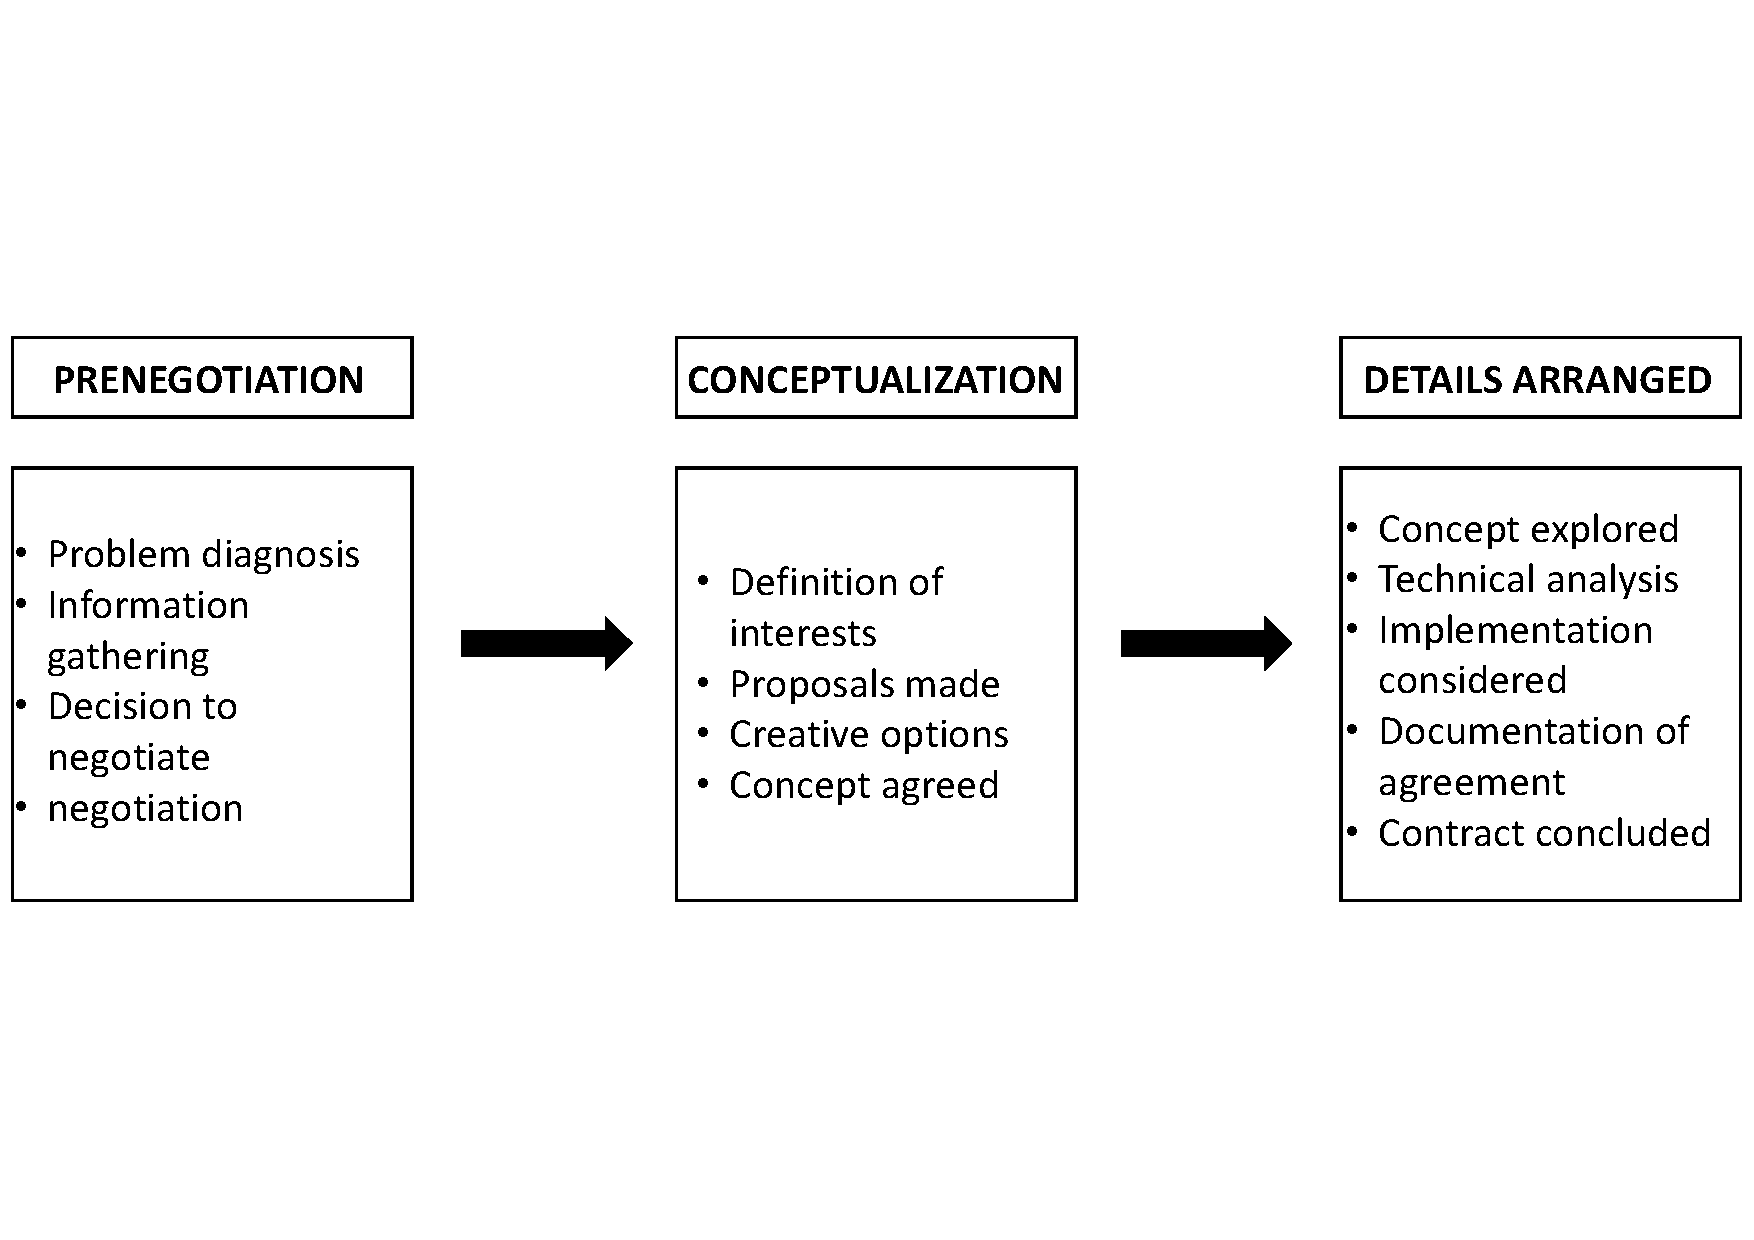
\includegraphics[trim={0 4,5cm 0 4,5cm},clip, width=\textwidth]{images/salacuse.pdf}
    \caption{Salacuse's Deal Making Process \mancite\autocite[19]{salacuse1}.}
\end{figure}

It is possible to notice how the concept of time influences the length of the first phase. Indeed, Asian cultures have a cyclical and long vision of time, where things take time to get done. Contrarily, Western cultures have a very fast paced concept of time, where what drives the negotiation is the agenda. Therefore, when negotiating together, Asian and Western culture may disagree on what takes more time. For Asian negotiators, it is very important to know their counterpart as they are relationship-oriented. Whereas Western negotiators are more interested in the substantive issue of the negotiation (for further references, see chapter 7). This will lead the two sides to spend more time on different stages, that is to influence their behaviours.\\
 
Another work that focuses on cultural influence in negotiations is "The Negotiation Dance: Time, Culture, and Behavioral Sequences in Negotiation" written by W. L. Adair and J. M. Brett. Their research starts with an example of dancing style to refer to the fact that, in negotiations, parties from different cultures will act differently, thus leading to inefficient negotiation outcomes. Indeed, they state that, when dancing, people from different countries will have different approaches to the same style (they report the example of ballroom dances: in Latin cultures, dancers will move more rapidly than their American counterparts, where ballroom dances are performed through smoother and lighter steps). Their work in divided in four main parts:
\begin{enumerate}
\item Four stage negotiation model;
\item Assertion of cultural influence on negotiators;
\item Prediction of particular stages that should originate efficient deals;
\item Testing the universal applicability of their hypothesis.
\end{enumerate}
Before continuing with their work, the authors provide us with a definition of behavioural sequences that negotiators use during a negotiation process: those are reciprocal sequences, complementary sequences, and structural sequences. Reciprocal sequences occur when negotiators respond to a cooperative (or competitive) behaviour with a similar behaviour. Complementary sequences exist when negotiators respond to "a cooperative or competitive behavior with a different but functionally similar behavior". Structural sequences "occur when negotiators use behaviours from different strategic groups" \autocite[35]{adair}.

\textbf{Stage model}.\\
The authors identify four main stages in a negotiation: relational positioning, identifying the problem, generating solutions, and reaching agreement \mancite\autocite[34]{adair}. 
\begin{itemize}
    \item \textit{Relational Positioning}. Adair and Brett assert that, at the beginning of the negotiation, parties can either be competitive or relationship-oriented. It is for this reason that negotiators "test" their opponents at first in order to assess whether they will be competitive (by trying to influence the opponents and by establishing a position) or cooperative (by disclosing little information about preferences and interests). Usually, most negotiations start with parties focusing on "influence with respect to status and power" \mancite\autocite[36]{adair}). Indeed, at the beginning of a negotiation, parties do not have knowledge of each others' interests, needs, and positions, therefore it would be difficult to rely on persuasive arguments. Negotiators use influence when they are trying to establish their power. However, as the negotiation continues, if negotiators keep relying on reciprocal persuasion, there will be the risk of a stalemate. The situation can be avoided when one of the parties take the leap of faith and discloses little information, as to signal the willingness to cooperate. That is when the process can continue.
    \item \textit{Identifying the Problem}. In the second stage, negotiators discuss about the details of the issues. During this phase, negotiators will exchange information in order to unveil interests, build trust, and seek an agreement.
    \item \textit{Generating Solutions}. During this stage, negotiators will try to create value and to claim value, therefore they will turn to a competitive approach again. Indeed, parties will make offers and counteroffers based on their own interests and priorities. The difference with the behaviour in Stage 1 is that this time negotiators know each others interests and therefore the persuasion will be based on rational reasoning rather than status.
    \item \textit{Reaching Agreement}. In this stage, negotiators will try to reduce the alternatives in order to identify an agreement. Thus, negotiators will make more and more offers and more and more concessions \mancite\autocite[37]{adair}. The negotiators will respond to offers with counteroffers rather than persuasive arguments. Because parties know each others' interests, the exchange of offers and counter offers foster the reaching of an agreement and the maximisation of the value each party gets from the agreement.
\end{itemize}

\textbf{Cultural influence on Negotiations}.\\
In order to assess the cultural influence on the negotiation stages, the authors appeal to Hall's theory of low/high context communication\footnote{Hall's work has already been cited in this thesis: for further references, see chapter 6.}.
In Western cultures, communication is direct, thus they are low-context cultures. On the other hand, Eastern cultures tend to have an indirect approach, thus being high-context cultures. In low-context communication, the meaning is clearly contained in the words; on the contrary, in high-context communication, the meaning is latent and has to be searched within the lines. As a consequence, in order to extract the meaning it is necessary to have deductive skills. Meanwhile, in low-context cultures, it is not necessary to have such skills.

Negotiators from high context cultures are expected to manage both high-context and low-context communications, while negotiators from low-context cultures will not be at ease with high-context communication. The authors assert that this fact will be noticeable in complementary sequences with behaviours with different level of directness. For example, affective persuasion suits a high context negotiator because it is indirect and refers to contextual factors, whereas rational influence (a complementary behaviour of affective persuasion) fits a low context negotiator, as it refers to facts and it is more direct \mancite\autocite[38]{adair}.

According to the authors, "complementary sequences define a culture-specific rhythm of the four-stage negotiation dance" \mancite\autocite[38]{adair}. But how?

Starting with the first stage, in which negotiators establish their positions, it is possible to assess that high-context negotiators will be more likely to "combine both direct, rational influence and indirect, affective influence in their positional sequences" \mancite\autocite[38]{adair} than low-context negotiators.

The second stage, in which the negotiators discuss about the issue by getting information, high-context negotiators are more likely to mix the communication approaches: they will use both direct statements (about priorities, for example) and indirect statements (about information, for example). Indeed, complementary sequences are "a signature rhythm of the high-context negotiation dance"\mancite\autocite[38]{adair}.

The low-context negotiator is not accustomed to high-context communication. Therefore, when negotiating with a high-context negotiator (so a mixed-context negotiation), it is difficult for them to be comfortable. Indeed, in mixed-context negotiations, high-context negotiators should avoid using high-context communication and switch to direct, low-context communication, which is the common denominator, the context everyone is comfortable using.

The stages that are more influenced by a cultural context are the first two. Indeed, communication-wise, high-context and low-context cultures have an opposite approach to express themselves. And where communication is key, it goes without saying that culture have an influence on how the negotiation will be conducted.\\

Culture can influence the negotiations under the stages approach. This chapter provided an insight of which ways culture influences the process of negotiation. The first article presented us the issue under the concept of time and relationship. The second article focused on communication by citing Hall's theory of low-context and high-context cultures.

\end{document}